\documentclass[12pt]{article}
\usepackage{graphicx} 
\usepackage{amsmath}
\usepackage{amsthm}
\usepackage{graphicx}
\usepackage{enumerate}
\usepackage{natbib}
\usepackage{booktabs}
\usepackage{hyperref}
\hypersetup{colorlinks = true, linkcolor = blue, citecolor=blue, urlcolor = blue}
\usepackage{enumitem}
\newcommand{\blind}{0}
\addtolength{\oddsidemargin}{-.5in}%
\addtolength{\evensidemargin}{-.5in}%
\addtolength{\textwidth}{1in}%
\addtolength{\textheight}{1.3in}%
\addtolength{\topmargin}{-.8in}%
\usepackage{float}
\usepackage{array} 



\begin{document}



\def\spacingset#1{\renewcommand{\baselinestretch}%
{#1}\small\normalsize} \spacingset{1}


%%%%%%%%%%%%%%%%%%%%%%%%%%%%%%%%%%%%%%%%%%%%%%%%%%%%%%%%%%%%%%%%%%%%%%%%%%%%%%

\if0\blind
{
  \title{\bf The usage of bootstrap method in shape-restricted regression}
  \author{Guanghong Yi\\
  Jun Yan\\[1ex]
  Department of Statistics, University of Connecticut\\
}
  \maketitle
} \fi

\if1\blind
{
  \bigskip
  \bigskip
  \bigskip
  \begin{center}
    {\LARGE\bf The usage of bootstrap method in shape-restricted regression}
\end{center}
  \medskip
} \fi

\bigskip
\begin{abstract}
The bootstrap method is an important resampling technique used to estimate statistics on a population by repeatedly sampling the data. It is also an effective approach for estimating the measure of dispersion in a dataset, especially in regression analysis. Meanwhile, the bootstrap method is also a valid method for constructing pointwise confidence intervals for time points in regressions. However, in some special cases, regression models need to be constrained with known characteristics such as monotonicity or curvature, for example, in growth curves, where the coefficients are forced to be non-negative. In such situations, spline regression is used for modeling. It is not always certain whether the bootstrap method can be directly applied to estimate the dispersion under these shape-restricted scenarios, especially for pointwise confidence intervals. In this article, we will demonstrate the usage of the bootstrap method in shape-restricted regression and proof the effectiveness of bootstrap for constructing pointwise confidence intervals in shape-restricted regression empirically.
\end{abstract}

\noindent%
{\it Keywords:}  bootstrap; shape-restricted regression; pointwise confidence interval; growth curve; splines regression
\vfill

\newpage
\spacingset{1.45} 
\section{Introduction}
\label{sec:intro}

In certain area and cases, apply shape restrictions, such as monotonicity or convexity to estimate a certain function is reasonable and not uncommon in many fields.\cite{guo2019smooth} There are several methods to build shape-restricted regressions to do analysis the regressions, like quadratic programming.\cite{meyer2013simple} However, due to shape restrictions, it is not quite accurate to estimate the uncertainty of the parameters with normal methods like MLE (Maximum likelihood estimation) since parameters will sometimes lies on the boundary. In this paper, we consider to use bootstrap method to replace MLE method to estimate the uncertainty of the parameters, specifically, of certain time points in the regression curve. Although the bootstrap method is a valid method used to construct confidence intervals for regression coefficients, \cite{efron1985bootstrap}and its effectiveness have been widely recognized in linear regression analysis \cite{efron1979bootstrap}, and non-linear regression analysis \cite{davidson1999bootstrap}. However, when dealing with shape-restricted regressions, where the coefficients are forced to adhere to specific constraints such as monotonicity or curvature, the effectiveness of bootstrap is not proved to be guaranteed. In this paper, we will demonstrate the usage of the bootstrap method in shape-restricted regression and proof the effectiveness of bootstrap for constructing pointwise confidence intervals in shape-restricted regression empirically. 

The rest of the paper is organized as the follows. Section~\ref{Bootstrap Method for Constructing Confidence Intervals} gives a review of bootstrap method for constructing confidence intervals. Section~\ref{Shape Restricted Example} gives out a shape-restricted regression example and the usage of bootstrap to build the pointwise confidence intervals for certain time points. Section~\ref{Simulation Study} shows a simulation study to assess the performance of the methods.
explores the case where a combination of the first two scenarios occurs. An  
adjusted bootstrap procedure is proposed as a working solution in this case.  
Section~\ref{Conclusion} concludes with a discussion.




\section{Bootstrap Method review}
\label{Bootstrap Method for Constructing Confidence Intervals}

The bootstrap is a powerful and important resampling method for estimating population parameters or assessing the accuracy of a statistical procedure by repeatedly sampling the data with replacement. Its effectiveness have been widely recognized in linear regression analysis \cite{efron1979bootstrap}, and non-linear regression analysis \cite{davidson1999bootstrap}. By bootstrap method, we can estimate the standard errors and confidence intervals for the regression coefficients. Even for unknown underlying population distributions, bootstrap method can resample the data with replacement and computes the regression coefficients for each resampled dataset. \cite{hall2013simple}By repeating this process many times, it provides a valid empirical estimate of the standard errors in both linear cases \cite{efron1985bootstrap} and nonlinear cases\cite{wong2019bootstrap}, thus it is valuable when the assumptions of traditional standard error estimation techniques are violated. It is also a valid method used to construct confidence intervals for regression coefficients. \cite{efron1985bootstrap}By resampling the dataset, bootstrap can determining the percentile intervals of these coefficients, and also can obtain approximate confidence intervals for the regression parameters. \cite{cui2012evaluating} Bootstrap can also construct the approximate confidence interval for certain time points f(t)s in the function by simulating f'(t) certain times in certain time points. \cite{horowitz2018bootstrap} Thus it is useful in regression analysis to estimate the uncertainty associated with the regression coefficients or for certain time points inside the regression function. \cite{Efron2011-sn}For convenience, in here we just talk about simple regression model which only contains one independent variable and one dependent variable. Specifically, the bootstrap method basically contains the following steps:

\begin{enumerate}[label=\arabic*.]
    \item Suppose we observed specific independent data points \(x_1, x_2, \ldots, x_n\) from a dataset, and for convenience we placed them inside a vector \(X = (x_1, x_2, \ldots, x_n)\), and since we want to construct a regression for the dataset, these data points are supposed to have a corresponding \(y\) values as dependent variable, and this makes the data points becomes pairs as \(X = (x_1,y_1) , (x_2,y_2),  \ldots, (x_n,y_n)\), and we call this as original dataset \(X\). Then we use the original dataset \(X)\) to create a simple regression model \(y = \beta_0 + \beta_1 x\).
    \item From the original dataset \(X\), generate \(n = B\) bootstrap samples, and placed them inside a dataset denoted as \(X^* = x_1^*, x_2^*, \ldots, x_n^*\), each bootstrap samples are obtained by sampling inside the original dataset \(X\) with replacement.
    \item With this bootstrap dataset, we can do the inference for any statistics we are interested in the original dataset. For exsample, if we are interested in the standard error \(s(x)\) for the original dataset, we may use the bootstrap dataset to inference it. The bootstrap estimate of standard error is the standard deviation calculated by the bootstrap dataset \(X^*\):
    \begin{equation}
      \hat{se_{boot}} = \{\sum_{b=1}^{B}[s(X^*)-s(*)]^2/(B-1)\}^{1/2}
    \end{equation}

    \item Using the data in the original sample dataset as the "population," perform nonparametric resampling with replacement to obtain a resampled sample (also known as the Bootstrap sample), denoted as \(x_1^*, x_2^*, \ldots, x_n^*\) (the number of data points in the Bootstrap sample must be the same as the number of data points in the original sample).
    \item If we are interested in confidence interval for certain regression coefficients or time points, we can also use bootstrap method to construct it, in this situation, \( [\hat{f}_n(t) - \hat{q}_{1-\alpha/2,n-1/3}, \hat{f}_n(t) - \hat{q}_{\alpha/2,n-1/3} ]\)  would be the bootstrap estimated pointwise confidence interval where \(\hat{q}_\alpha\) denoted the \(\alpha\)th quantile of the time point \(t\).

\end{enumerate}

Bootstrap method has been proved that it is an excellent method to estimate statistic \cite{efron1979bootstrap}, the \(u^*\) we obtained from the resampling dataset is a good estimator for the \(v\) as a population parameter. According to the bootstrap method, we can also calculate the confidence interval for the parameters, or the coefficients of a certain regression, or for certain time points in the regression. In this article, we will focus on the method of construct a pointwise confidence interval by bootstrap. It has been proved that the bootstrap method can be used as a good estimator for the pointwise confidence interval in linear regressions and non-linear regressions\cite{efron1979bootstrap}\cite{davidson1999bootstrap}, and some examples in certain configurations are given.\cite{ruhe2019bootstrap}\cite{ma2019inference}\cite{dugas2010pointwise} But in certain special cases(i.e. shape-restricted splines regressions) there is no certain resource have not prove that it is a good method to build pointwise confidence interval via bootstrap.

Shape-restricted splines regressions are piecewise polynominal, differentiable to a certain degree and have certain restrictions like monotonicity or convexity.\cite{meyer2008inference} Given these conditions, the application of the bootstrap method to estimate pointwise confidence intervals for specific time points within the regression cannot be guaranteed to be suitable. And in the rest of the article we gives out an example of shape-restricted regression and the method to fit confidence interval for certain time points in the function.









\section{Shape Restricted Example}
\label{Shape Restricted Example}

In some situations the regression is forced to be shape-restricted to improve the predictive performance and reduce overfitting if the underlying regression function takes the specific form. Some regressions are naturally constrained to convexity or concativity in a lot of disciplines like economics, biology, and psychological studies, and other ares.\cite{jieying2022heteroscedastic} \cite{guntuboyina2018nonparametric} Some popular examples like cost function and profit function in economics\cite{gallant1984imposing}, precipitation data analysis\cite{molitor2002bayesian}. In this article we gives out an example of the relationship between income and the age of Canadian workers. The data is given from R package SemiPar. For those situations, Regression splines are smooth, flexible, and parsimonious nonparametric function estimators, and it offers an effective approach to enhance the inference of shape-restricted regression. \cite{meyer2008inference} In this dataset, a nondecreasing relationship between the age of workers and the expected logarithm of the income was considered. \cite{wang2021shape}  Splines2 provides implementation of those spline basis functions via R language, and we use that to build a non-decreasing curve by i-spline that force the coefficients to be non-negative with degree of freedom = 6. Then, we selected 10 time points, denoted as $t$, with equal intervals from the dataset, corresponding to one of them is the regression time points \(f'(t)\) that fitted by iSpline. We also performed bootstrap resampling 1000 times to obtain the 95\% quantile pointwise confidence interval for each points. In the figure below, the red line represents the fitted i-spline regression, the yellow line is the smooth regression, and we build ten pointwise confidence intervals for 10 certain time points. The result is shown in Figure ~\ref{fig:semipar}.


\begin{figure}[H]
  \centering
  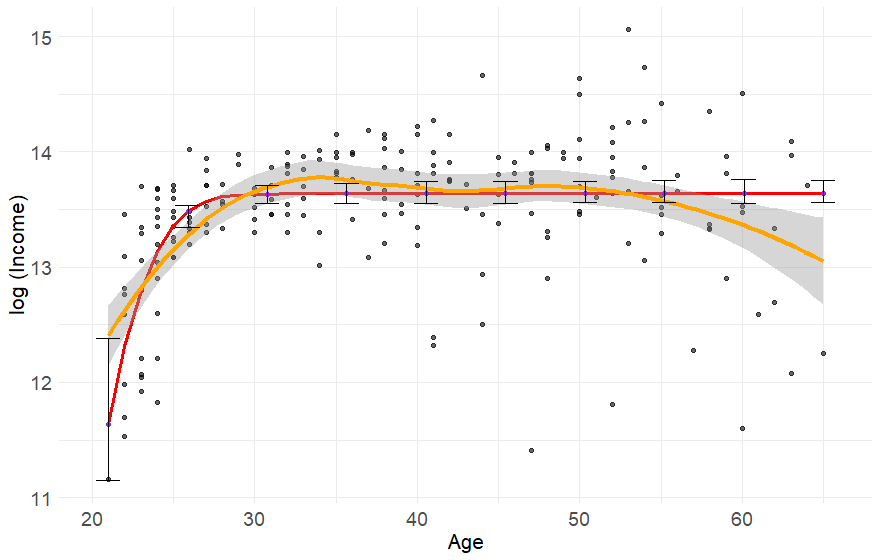
\includegraphics[width=0.8\textwidth]{SemiparCI.png}
  \caption{CI build for the shape-restricted regression: The red line is the fitted i-splines regression, the yellow line is the smoothing splines, the grey area represents the \(95\%\) confidence interval for the smoothing splines, and the black solid intervals are the bootstrap pointwise confidence intervals for certain time points. }
  \label{fig:semipar}
\end{figure}

We can see that, for this one-time example all the pointwise confidence intervals constructed by the bootstrap method include the fitted regression. But it is not a valid proof that bootstrap is a good method for constructing pointwise confidence intervals since the regression is fitted by the dataset, and the criteria is given by \(f'(t)\) which is given by the regression but not the the true value \(f(t)\). In this case, a simulation study is required to further prove the effectiveness of bootstrap pointwise confidence intervals.









\section{Simulation Study}
\label{Simulation Study}


Since the underlying distribution is unknown, we need to perform a simulation study to test whether the fitted pointwise confidence interval is accurate for the regression.


We define three functions: \(y = 0.25(x - 0.9)\) , \(y = 0.02(x^3+1.2)\) , and \(y = 0.1(5\Phi((x - 2)/0.3) + 1)\) , where \(\Phi\) is the cumulative distribution function of the standard normal distribution. For those functions, the validity of the bootstrap method to build the confidence intervals for the coefficients and standard error has already been proved. \cite{jieying2022heteroscedastic} And in this article we want to further prove the validity of the bootstrap method to build the pointwise confidence intervals for certain time points in the domain of the function. First of all, we randomly generate some data points \(x\) in the domain of \([0,4]\), and we calculate its corresponding values \(y(x)\), and make simulation data points \(f'(x)\) by add noise to the true value \(f(x)\). The noise is added from a standard normal distribution with \(\mu = 0\) and \(\sigma = \) \(1\). And then we make the paired values \((x, y\text{ with noise})\) be the dataset, while we know the true values of \(f(x)\) as well. 


\begin{figure}[H]
  \centering
  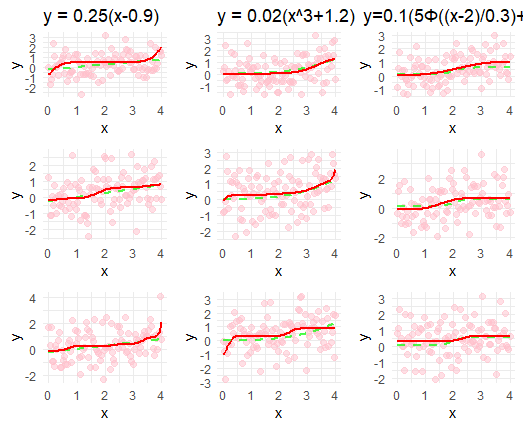
\includegraphics[width=0.8\textwidth]{DataPointsGeneration.png}
  \caption{The generated dataset while n=100, true functions and fitted i-splines regressions: the shaded green curve represents the true functions, the pink points are the data pair \((x, f'(x))\) where \(f'(x)\) is generated by \(f(x)\) add noise, and the red curves are the fitted i-splines regression curve with degrees of freedom\(= 6,10,15\), from top to bottom}
  \label{fig:DataAndRegressions}
\end{figure}

We use quadratic i-splines function to enforce the monotonicity of the function and we picked degrees of freedom 6 and 10 to build the regression for the dataset. The generated dataset and regressions is shown in Figure ~\ref{fig:DataAndRegressions}. While according to the law of large number, we also expect that the result will be closer to \(95\%\) while n gets larger, so we also did a simulation for \(n = 1000\) to see the numeric coverage percentiles. In each configuration, we select \(0.5,1,1.5,2,2.5,3,3.5,4\) as the time points from the dataset and perform bootstrap resampling 1000 times to estimate the \(95\%\) quantile pointwise confidence intervals for each of the selected time points. We repeat this process 1000 times to see how many times these confidence intervals can contain the true result. The results are shown in Table ~\ref{Table} and Table ~/ref{2}. 



\begin{table}[ht]
  \centering
  \caption{Results for Different Degrees of Freedom (\(n = 100\))}
  \label{Table1}
  \begin{tabular}{|c|c|c|c|}
    \hline
    \textbf{x} & \textbf{Function} & \textbf{CP of df\_6} & \textbf{CP of df\_10} \\
    \hline
    \multicolumn{4}{|c|}{\(y = 0.25(x - 0.9)\)} \\
    \hline
    0.5 & -0.100 & 0.952 & 0.959 \\
    \hline
    1.0 & 0.025 & 0.956 & 0.948 \\
    \hline
    1.5 & 0.150 & 0.959 & 0.940\\
    \hline
    2.0 & 0.275 & 0.956 & 0.953 \\
    \hline
    2.5 & 0.400 & 0.952 & 0.957 \\
    \hline
    3.0 & 0.525 & 0.950 & 0.953 \\
    \hline
    3.5 & 0.650 & 0.945 & 0.950 \\
    \hline
    4.0 & 0.775 & 0.926 & 0.908 \\
    \hline
    \multicolumn{4}{|c|}{\(y = 0.02(x^3+1.2)\)} \\
    \hline
    0.5 & 0.027 & 0.938 & 0.937 \\
    \hline
    1.0 & 0.044 & 0.946 & 0.952 \\
    \hline
    1.5 & 0.092 & 0.932 & 0.943 \\
    \hline
    2.0 & 0.184 & 0.936 & 0.945 \\
    \hline
    2.5 & 0.337 & 0.942 & 0.948 \\
    \hline
    3.0 & 0.564 & 0.960 & 0.946 \\
    \hline
    3.5 & 0.882 & 0.940 & 0.943 \\
    \hline
    4.0 & 1.304 & 0.907 & 0.907 \\
    \hline
    \multicolumn{4}{|c|}{\(y = 0.1 (5\Phi((x - 2) / 0.3) + 1)\)} \\
    \hline
    0.5 & 0.100 & 0.938 & 0.947 \\
    \hline
    1.0 & 0.100 & 0.927 & 0.941 \\
    \hline
    1.5 & 0.124 & 0.826 & 0.830 \\
    \hline
    2.0 & 0.350 & 0.962 & 0.958 \\
    \hline
    2.5 & 0.576 & 0.835 & 0.816 \\
    \hline
    3.0 & 0.600 & 0.935 & 0.945 \\
    \hline
    3.5 & 0.600 & 0.957 & 0.953 \\
    \hline
    4.0 & 0.600 & 0.875 & 0.840 \\
    \hline
  \end{tabular}
\end{table}


\begin{table}[ht]
  \centering
  \caption{Results for Different Degrees of Freedom (\(n = 1000\))}
  \label{Table2}
  \begin{tabular}{|c|c|c|c|}
    \hline
    \textbf{x} & \textbf{Function} & \textbf{CP of df\_6} & \textbf{CP of df\_10} \\
    \hline
    \multicolumn{4}{|c|}{\(y = 0.25(x - 0.9)\)} \\
    \hline
    0.5 & -0.100 & 0.956 & 0.948 \\
    \hline
    1.0 & 0.025 & 0.953 & 0.957 \\
    \hline
    1.5 & 0.150 & 0.961 & 0.955 \\
    \hline
    2.0 & 0.275 & 0.967 & 0.955 \\
    \hline
    2.5 & 0.400 & 0.956 & 0.953 \\
    \hline
    3.0 & 0.525 & 0.949 & 0.961 \\
    \hline
    3.5 & 0.650 & 0.952 & 0.946 \\
    \hline
    4.0 & 0.775 & 0.952 & 0.937 \\
    \hline
    \multicolumn{4}{|c|}{\(y = 0.02(x^3+1.2)\)} \\
    \hline
    0.5 & 0.027 & 0.964 & 0.961 \\
    \hline
    1.0 & 0.044 & 0.950 & 0.954 \\
    \hline
    1.5 & 0.092 & 0.937 & 0.939 \\
    \hline
    2.0 & 0.184 & 0.939 & 0.949 \\
    \hline
    2.5 & 0.337 & 0.947 & 0.952 \\
    \hline
    3.0 & 0.564 & 0.952 & 0.946 \\
    \hline
    3.5 & 0.882 & 0.961 & 0.950 \\
    \hline
    4.0 & 1.30 & 0.963 & 0.936 \\
    \hline
    \multicolumn{4}{|c|}{\(y = 0.1 (5\Phi((x - 2) / 0.3) + 1)\)} \\
    \hline
    0.5 & 0.100 & 0.956 & 0.934 \\
    \hline
    1.0 & 0.100 & 0.936 & 0.912 \\
    \hline
    1.5 & 0.124 & 0.956 & 0.373 \\
    \hline
    2.0 & 0.350 & 0.967 & 0.951 \\
    \hline
    2.5 & 0.576 & 0.956 & 0.411 \\
    \hline
    3.0 & 0.600 & 0.954 & 0.905 \\
    \hline
    3.5 & 0.600 & 0.951 & 0.922 \\
    \hline
    4.0 & 0.600 & 0.946 & 0.837 \\
    \hline
  \end{tabular}
\end{table}


In table ~\ref{Table1}, \(x\) represents the certain time point we selected in the domain of the function, and \(f(x)\) is its true value calculated by the certain known function. CP represents coverage percentage of pointwise confidence interval we built by the bootstrap methods under certain degrees of freedom. We can see that in all those functions and degrees of freedom we have given, the bootstrap method gives pointwise confidence intervals coverage that are closed to the nominal level \(95\%\). And we can also see that while n gets larger, the result of \(n = 1000\), which can be seen in Table ~\ref{Table2} is much better than \(n = 100\) in each same level of degrees of freedom. While degrees of freedom is also an important variable inside the study and we can see that for the different degrees of freedom the result of CP is different either, but since it is not the main scope of this paper, we will not concern a lot about how to choose the best model to enhence the CP result.

\section{Conclusion}
\label{Conclusion}
In this study, we explored the application of the bootstrap method of building pointwise confidence intervals in shape-restricted cases. We demonstrated its effectiveness in constructing pointwise confidence intervals for certain time points within the regression function. 

We gives out a simulation study to prove that the pointwise confidence intervals constructed using the bootstrap method provide good empirical coverage for the true values of the regression function. This suggests that the bootstrap method is a valid approach for enhancing the inference of shape-restricted regressions, even for pointwise confidence intervals.

Our findings support the utility of the bootstrap method to build the pointwise confidence intervals in cases where regression models have specific constraints such as monotonicity or curvature. However, it's important to consider the assumptions and limitations of the bootstrap method and validate its performance for specific datasets and applications.

\bibliographystyle{plain}
\bibliography{citations}

\end{document}